


\begin{frame}{So sánh $\epsilon$ objective và $\bx_0$ objective}
%$z_t = \sqrt{\bar{\alpha}_t}z_0 + \sqrt{1-\bar{\alpha}_t}\epsilon, \quad \epsilon \sim \mathcal{N}(0,I)$
%
%
%%$x_{t-1} = \sqrt{\alpha_{t-1}}\hat{x}_0 + \sqrt{1-\alpha_{t-1}}\epsilon$
%
%$\hat{z}_0 = f_\theta(z_T, t, \text{text\_embedding})$
%
%$L = \mathbb{E}_{t,z_0,\epsilon}[\|\hat{z}_0 - z_0\|_2^2]$
%
%$z_{t-1} = \sqrt{\alpha_{t-1}}\hat{z}_0 + \sqrt{1-\alpha_{t-1}}\epsilon$

\begin{figure}
	\centering
	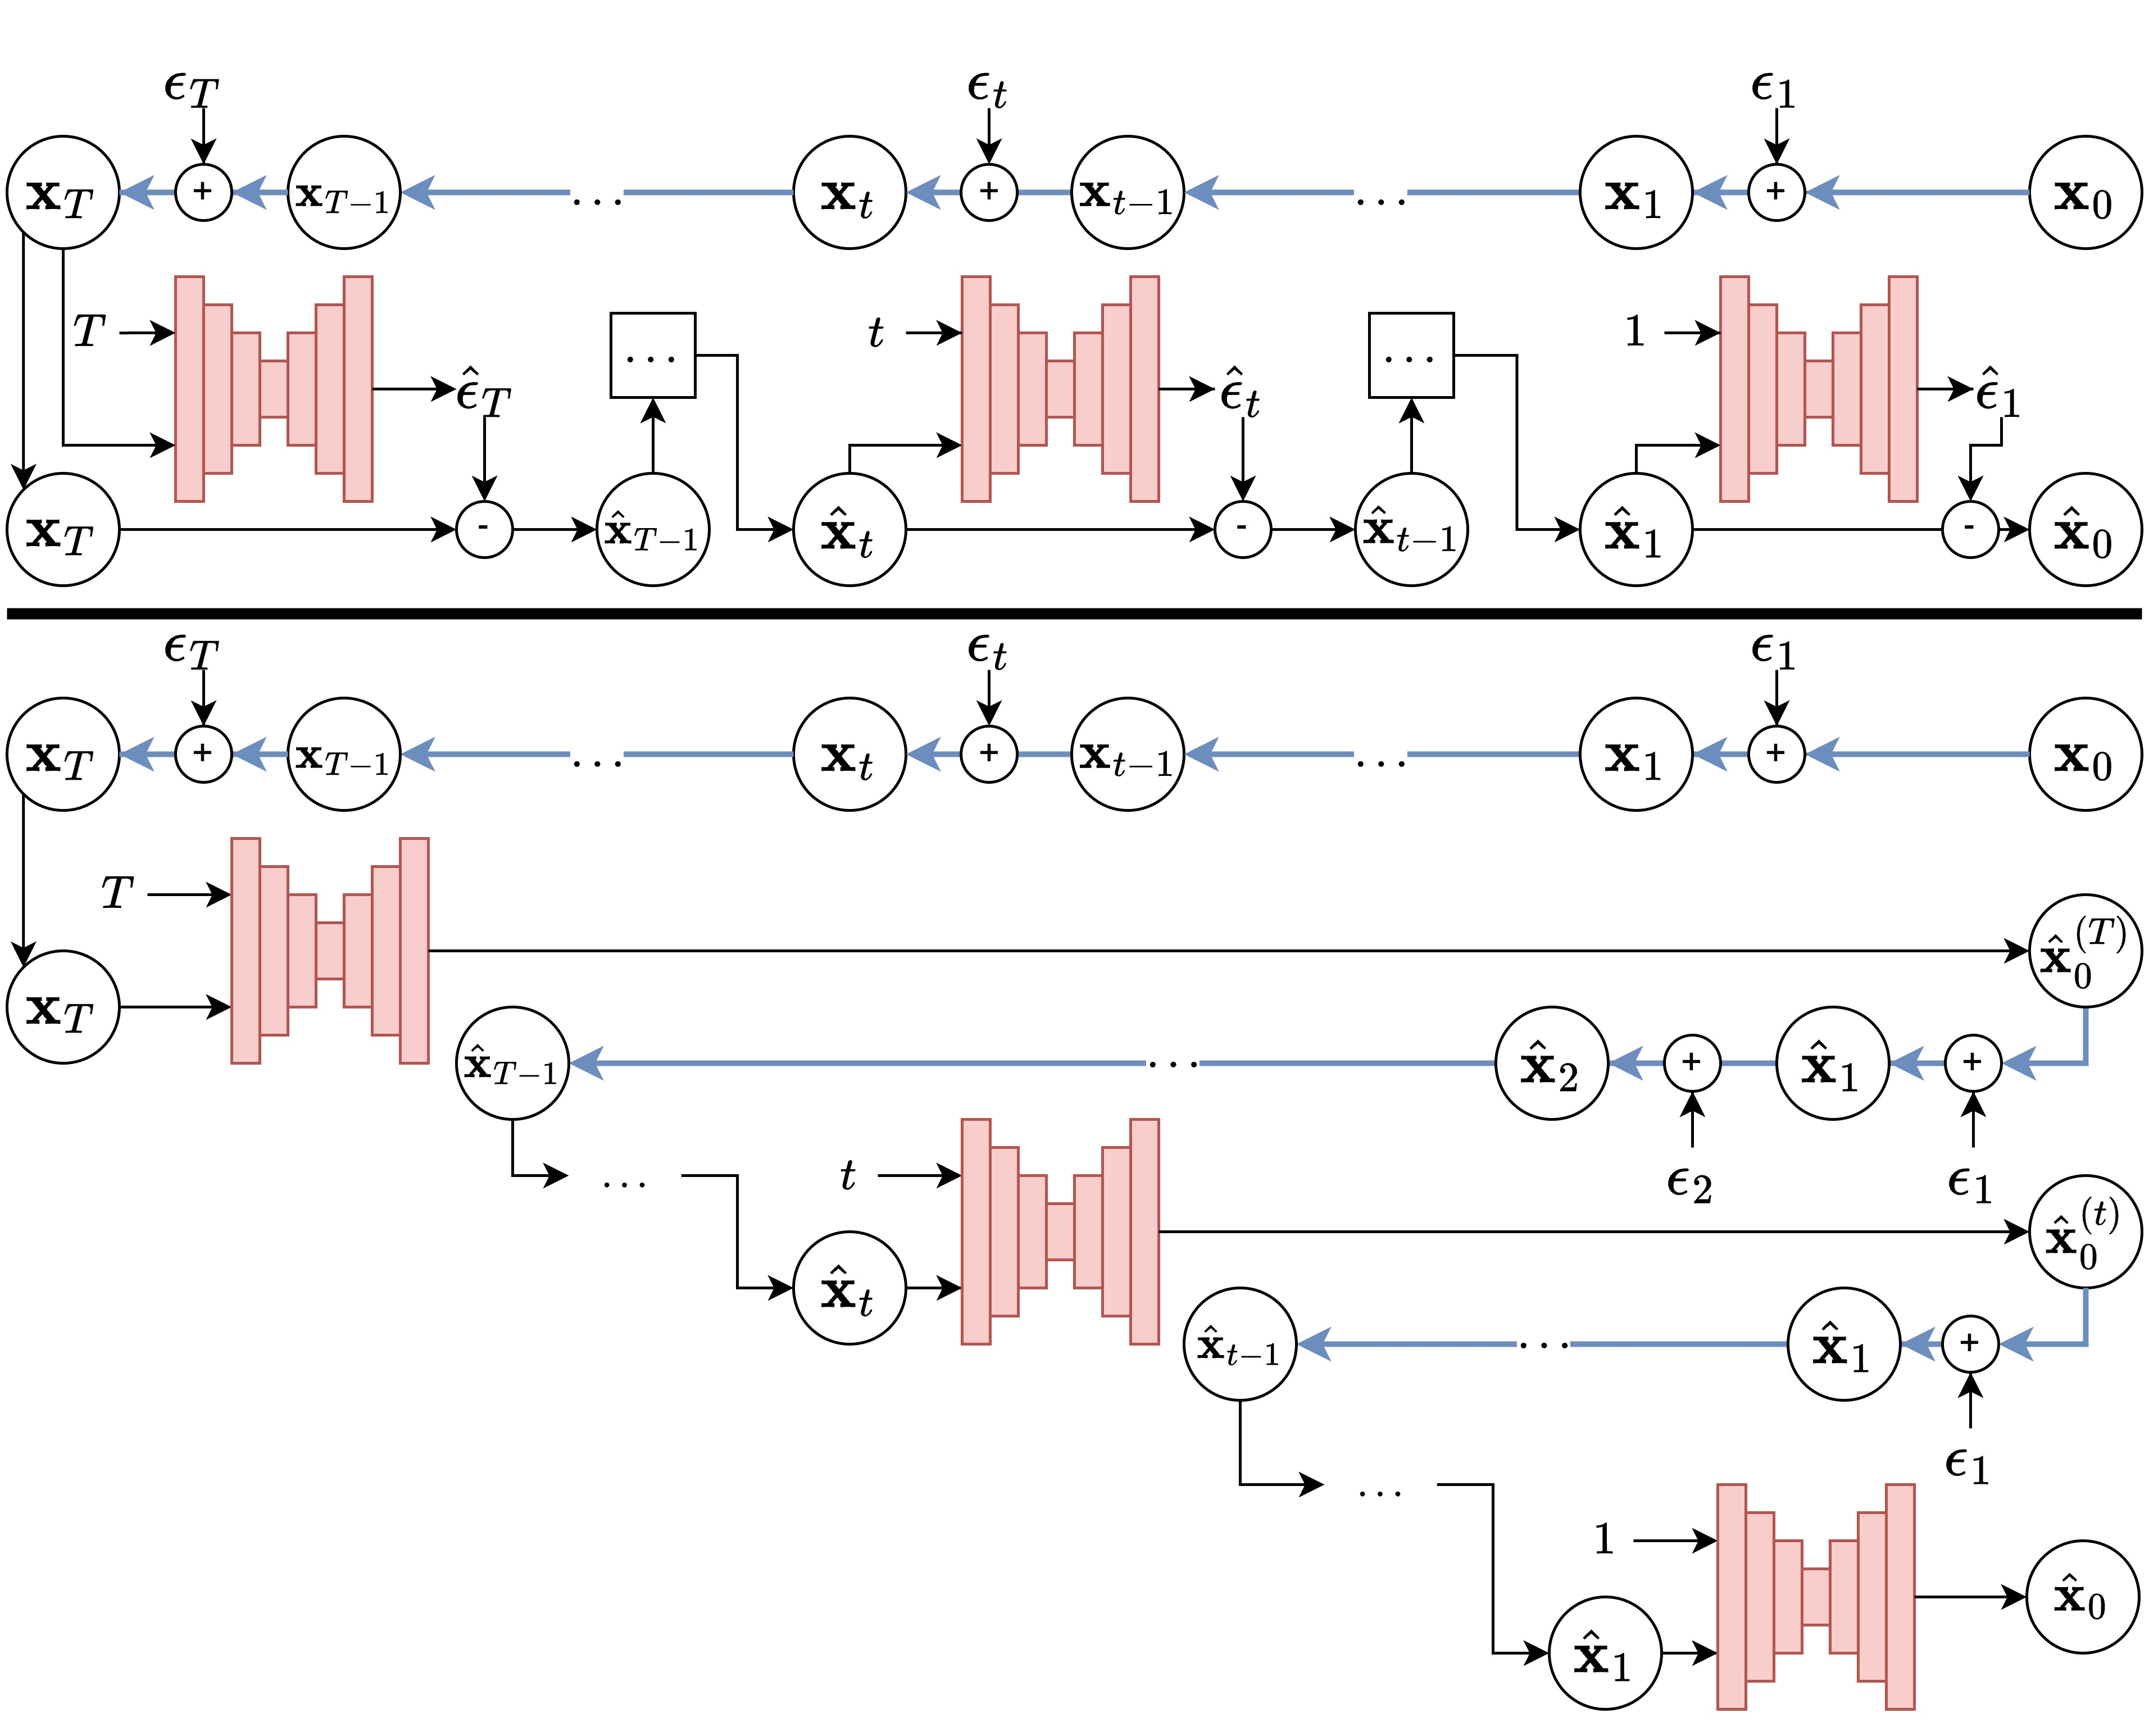
\includegraphics[width=0.95\linewidth]{X0Objective}
\end{figure}




%	
%	{Forward Process}
%	
%	\textbf{DDPM:}
%	\begin{equation}
%		q(x_t|x_{t-1}) = \mathcal{N}(x_t; \sqrt{1-\beta_t}x_{t-1}, \beta_tI)
%	\end{equation}
%	Trong đó:
%	\begin{itemize}
%		\item $\beta_t$ là lịch nhiễu (noise schedule)
%		\item $x_t$ là ảnh ở bước $t$
%		\item $\mathcal{N}$ là phân phối chuẩn (Gaussian)
%	\end{itemize}
%	
%	\textbf{DDIM:}
%	\begin{equation}
%		q(x_t|x_0) = \mathcal{N}(x_t; \sqrt{\bar{\alpha}_t}x_0, (1-\bar{\alpha}_t)I)
%	\end{equation}
%	Trong đó:
%	\begin{itemize}
%		\item $\bar{\alpha}_t = \prod_{i=1}^t(1-\beta_i)$
%		\item $x_0$ là ảnh gốc
%	\end{itemize}
%$x_t = \sqrt{\alpha_t}x_{t-1} + \sqrt{1-\alpha_t}\epsilon$

%\text{Trong đó:}
%\begin{align*}
%	& x_t: \text{là trạng thái tại thời điểm } t \\
%	& x_{t-1}: \text{là trạng thái tại thời điểm } t-1 \\
%	& \alpha_t: \text{là tham số variance scheduling } (0 < \alpha_t < 1) \\
%	& \epsilon \sim \mathcal{N}(0,1): \text{là nhiễu Gaussian}
%\end{align*}
%
%% Có thể viết dưới dạng tích lũy \bar{\alpha}
%$\text{Định nghĩa: } \bar{\alpha_t} = \prod_{i=1}^t \alpha_i$
%
%$x_t = \sqrt{\bar{\alpha_t}}x_0 + \sqrt{1-\bar{\alpha_t}}\epsilon$

%	$$\bx_{t-1} = \sqrt{\alpha_{t-1}} \left( \frac{\bx_t - \sqrt{\alpha_t} \epsilon_{\theta}(\bx_t, t)}{\sqrt{1 - \alpha_t}} \right) + \sqrt{1 - \alpha_{t-1}} \epsilon_{\theta}(\bx_t, t)$$
\end{frame}